% REGULAR GRAPH

\documentclass[border=5]{standalone}

\usepackage{tikz}

\begin{document}

    Graph 1:
    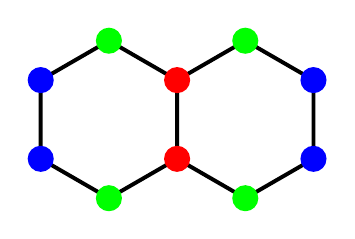
\begin{tikzpicture}[
            scale = 1,
            every node/.style={transform shape, text depth=0pt, circle},
            line/.style={line width = .05cm},
            ]
        \draw[line] (90:0.5cm) node[fill=red] {} -- ++ (150:1cm) node[fill=green] {} -- ++(210:1cm) node[fill=blue] {} -- ++(270:1cm) node[fill=blue] {} -- ++(330:1cm) node[fill=green] {} --++ (30:1cm) node[fill=red] {} --++ (90:1cm) -- ++(30:1cm) node[fill=green] {} -- ++(330:1cm) node[fill=blue] {} --++(270:1cm) node[fill=blue] {} --++(210:1cm) node[fill=green] {} --++(150:1cm) ;
    \end{tikzpicture}
    
    Graph 2:
    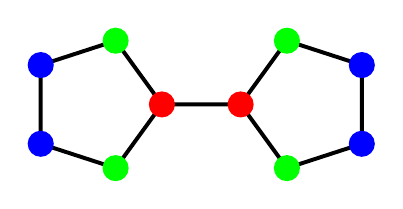
\begin{tikzpicture}[
            scale = 1,
            every node/.style={transform shape, text depth=0pt, circle},
            line/.style={line width = .05cm},
            ]
        
        \draw[line] (0:1cm) node[fill=red] {} --++(180-54:1cm) node[fill=green] {} --++(270-72:1cm) node[fill=blue] {} --++(270:1cm) node[fill=blue] {} --++(-18:1cm) node[fill=green] {} --++(90-36:1cm) --++(0:1cm) node[fill=red] {} --++(54:1cm) node[fill=green] {} --++(-18:1cm) node[fill=blue] {} --++(270:1cm) node[fill=blue] {} --++(180+18:1cm) node[fill=green] {} --++(90+36:1cm);
        
        
    \end{tikzpicture}
    
\end{document}